
\documentclass{article}

\usepackage{lipsum} 
\usepackage{graphicx}
\usepackage{subcaption}
\usepackage{multirow}
\usepackage{float}

\graphicspath{ {./} }

% \usepackage[bottom=2in]{geometry}


\usepackage{amsmath}
\usepackage{mathtools}
% \usepackage{}

\newcommand{\deriv}[1]{\frac{d#1}{dx}}

\begin{document}

\title{CSE200: Online-1 on \LaTeX}

\author{Mehedi Hasan Kanon (202305052)}

\date{Jane 26, 2026}

% IMPORTANT to use this command here
\maketitle

\section{Introduction}
Document preparation systems are essential for producing structured and professional technical documents. \textbf{LATEX} allows authors to focus on content while maintaining consistent formatting. This article demonstrates formatted text, lists, equations, tables, and figures using commands taught in class.

\subsection{Text Emphasis and Fonts}
This sentence contains \textbf{bold text}, \textit{italic text}, \emph{emphasized text}, and \underline{underlined text}. Font sizes can also vary such as {\large Large text}, {\small small text}, and {\huge huge text}.


\section{List Structures}

\subsection{Mixed and Nested Lists}

\begin{itemize}
    \item Primary Feature
    \item Secondary Feature
    \begin{enumerate}
        \item Formatting control
        \item Mathematical typesetting
        \begin{itemize}
            \item[--] Inline math
            \item[--] Display math 
        \end{itemize}
    \end{enumerate}
    \item[\textbf{Note}] Lists can be customized
\end{itemize}

\section{Mathematical Modeling}

Mathematical expressions are often used to represent data relationships. Consider variables $x_i$, $y$ and $z^2$.

\section{Mathematical Modeling}
Mathematical expressions are commonly used to describe relationships among variables. Let the variables be $x_i$, $y_j$ and $\sigma^2$.

\subsection{Dsiplayed Equations}
\[y_j = \alpha x_{j}^{2} + \beta x_j + \gamma \tag{1}\]

\begin{align*}
    T &= \sum_{i = 1}^{n} \left( x_i - \mu \right)^2 \\
    &= \sum_{i = 1}^{n} x_i^2 - 2 \mu \sum_{i = 1}^{n} x_i + n \mu^2 \tag{2}
\end{align*}

\[ f(x_i) = \begin{cases*}
    \frac{x_i^2}{\sigma^2} & \text{if} $x_i \geq 0$  \\
    \frac{ \left| x_i \right|}{\sigma} & \text{if} $x_i < 0$  \\
\end{cases*}
\]

\section{Tabular Data Presentation}


\section{Visual Comparison}

\subsection{Asymmetric Subfigure Layout}
\begin{figure}[H]
    \centering
    \begin{subfigure}[b]{0.6\textwidth}
        \centering
        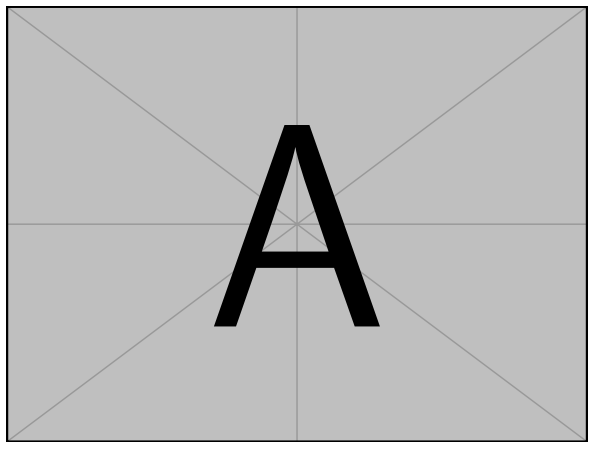
\includegraphics[width=\linewidth]{A.PNG}
        \caption{Main Diagram}
        \label{sub:main}
    \end{subfigure}
    % \hfill
    % \par\vspace{1em} 
    \par\medskip
    \begin{subfigure}[b]{0.31\textwidth}
        \centering
        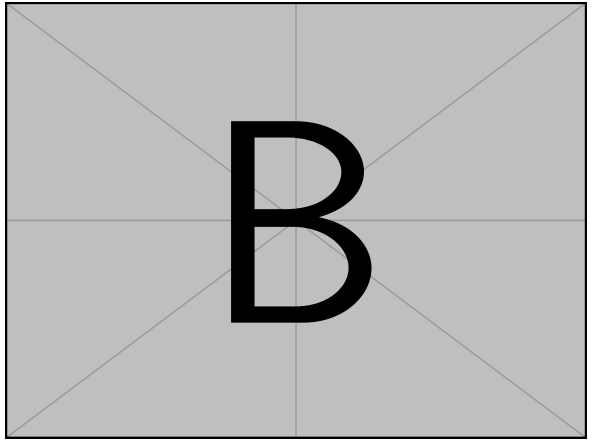
\includegraphics[width=\linewidth]{B.PNG}
        \caption{Detail B}
        \label{sub:det_b}
    \end{subfigure}
    \hfill
    \begin{subfigure}[b]{0.31\textwidth}
        \centering
        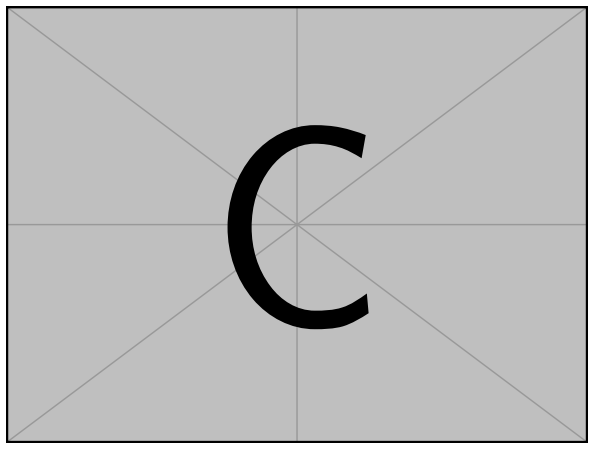
\includegraphics[width=\linewidth]{C.PNG}
        \caption{Detail C}
        \label{sub:det_c}
    \end{subfigure}

    \caption{Asymmetric layout with one dominant figure.}
    \label{fig:asymmetric_layout}

\end{figure}

% \begin{figure}[H]
%     \centering
    
%     % --- Top Row: One Dominant Figure ---
%     \begin{subfigure}[b]{0.6\textwidth}
%         \centering
%         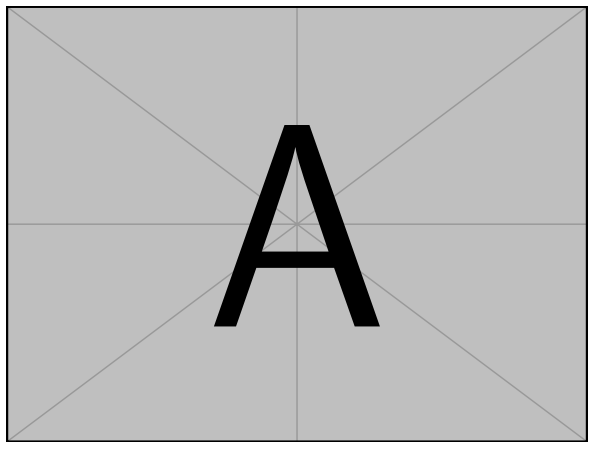
\includegraphics[width=\linewidth]{A.PNG}
%         \caption{Main Diagram}
%         \label{sub:main}
%     \end{subfigure}
    
%     \par\medskip
%     % \par\vspace{1em} % <--- CRITICAL: Forces a line break and adds a little vertical space
    
%     % --- Bottom Row: Two Side-by-Side Figures ---
%     \begin{subfigure}[b]{0.31\textwidth}
%         \centering
%         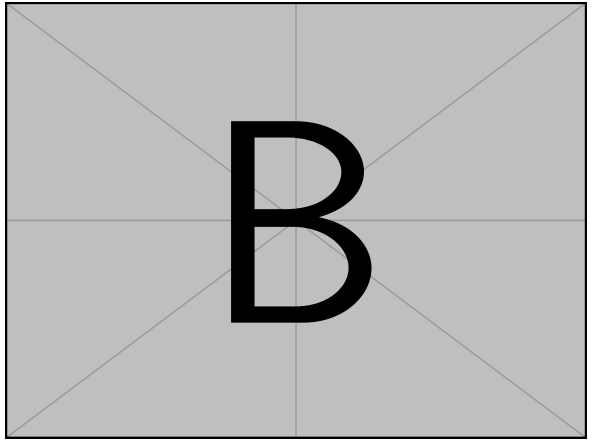
\includegraphics[width=\linewidth]{B.PNG}
%         \caption{Detail B}
%         \label{sub:detail_b}
%     \end{subfigure}
%     \hfill % Pushes the two bottom subfigures to opposite sides
%     \begin{subfigure}[b]{0.31\textwidth}
%         \centering
%         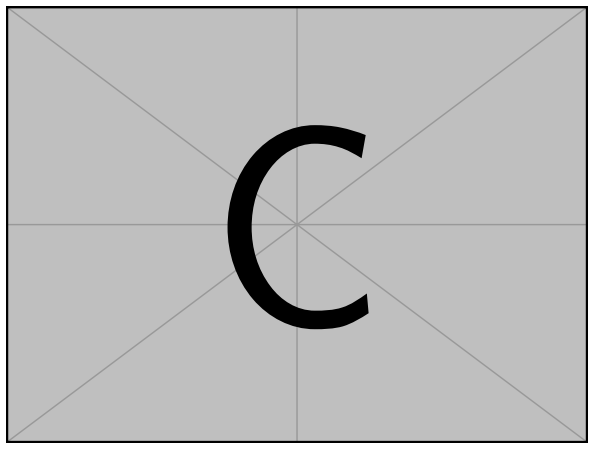
\includegraphics[width=\linewidth]{C.PNG}
%         \caption{Detail C}
%         \label{sub:detail_c}
%     \end{subfigure}

%     \caption{Asymmetric layout with one dominant figure.}
%     \label{fig:asymmetric_layout}
% \end{figure}

\noindent Figure 1 illustrates how visual elements can be arranged systematically within a document.

\section{Conclusion}

This article highlighted the importance of \textbf{structured writing} using \LaTeX. The use of \textit{formatted text}, mathematical expressions, tables, and figures improves both \underline{readability} and presentation quality. 

\end{document}